\documentclass{beamer}
\usepackage{xcolor}
\usepackage{graphicx}
\usepackage{CJKutf8}
\usepackage{listings}
\usepackage{underscore}
\usepackage[bookmarks=true]{hyperref}
\usepackage[utf8]{inputenc}
\usepackage[english]{babel}
\usetheme{Madrid}

\setbeamertemplate{footline}
{
\leavevmode
\hbox{
\begin{beamercolorbox}
[wd=1\paperwidth,ht=2.25ex,
dp=1ex,right]{date in head/foot}
\insertframenumber{} /
\inserttotalframenumber\hspace*{2ex}
\end{beamercolorbox}
}\vskip0pt
}

\AtBeginSubsection[]
{
  \begin{frame}<beamer>[shrink]{Outline}
    \tableofcontents[currentsection,currentsubsection]
  \end{frame}
}


\begin{document}
\begin{CJK}{UTF8}{nkai}
\title{開放平台軟體 期末報告}
\author{張友澤,李政憲,游登翔,張哲郡,劉彥麟}

\begin{frame}
  \titlepage
\end{frame}

\begin{frame}[shrink]{Outline}
  \tableofcontents
\end{frame}


\section{ Introduction}
\subsection{Introduction to your team}
\subsection{Introduction to the problem you're trying to solve}

\section{Methodology}
\subsection{Input of your model}
\subsection{Output of your model}
\subsection{Each layer of your model}
\subsection{How you save your model?}
\subsection{File size of your model}
\subsection{What's your loss functions, and why?}
\subsection{What's your optimizer and the setting of hyperparameter?}

\section{ Dataset}
\subsection { The size of our dataset should be larger than 1K}
\begin{frame}{Dataset}{The size of our dataset should be larger than 1K}
\begin{figure}
\begin{center} 
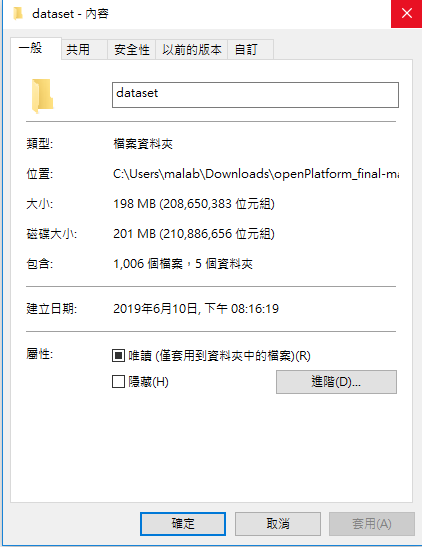
\includegraphics[height=4cm]{1.png}
\end{center}
\caption{It's our Datasize} 
\end{figure}
\end{frame}
\subsection{How you collect/build  dataset?}
\begin{frame}{Dataset}{How you collect/build  dataset?}
1.把音樂下載成MP3的格式
\newline
\newline
\newline
2.用裁切軟體裁剪成每10秒一個人聲的音訊檔
\newline
\newline
\newline
3.把這些資料取mfcc特徵向量並製作成.npy壓縮檔
\end{frame}
\subsection{How many paired training samples in dataset?}
\begin{frame}{Dataset}{How many paired training samples in  dataset?}
 使用800筆資料去訓練成模組
\newline
\newline
\begin{figure}
\begin{center} 
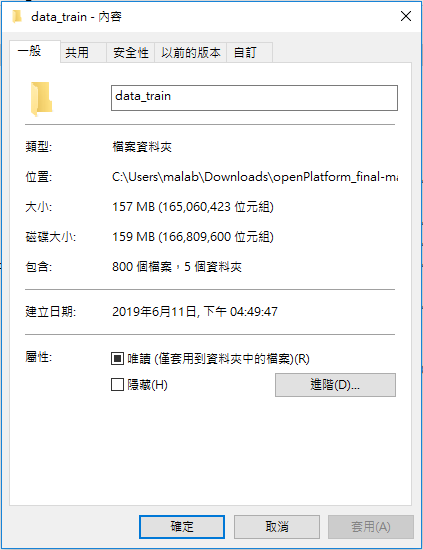
\includegraphics[height=4cm]{2.png}
\end{center}
\caption{所有類別的Train Data}
\end{figure}
\end{frame}
\subsection{How many paired validating samples in dataset?}
\begin{frame}{Dataset}{How many paired validating samples in  dataset?}
總共200筆資料來驗證模組的準確度
\newline
\newline
\begin{figure}
\begin{center} 
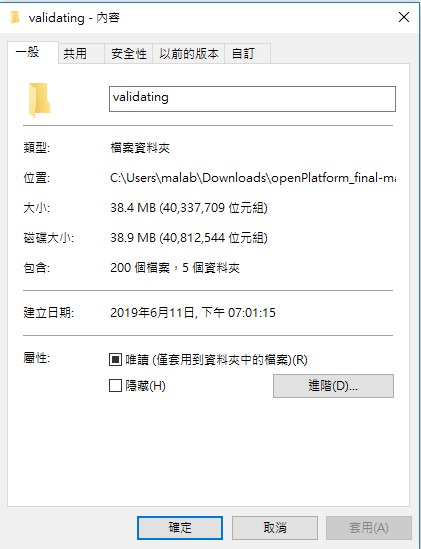
\includegraphics[height=4cm]{7.png}
\end{center}
\caption{所有類別的Validating Data}
\end{figure}
\end{frame}
\subsection{How many paired testing samples in  dataset?}
\begin{frame}{Dataset}{How many paired testing samples in  dataset?}
總共200筆資料來測試模組
\newline
\newline
\begin{figure}
\begin{center} 
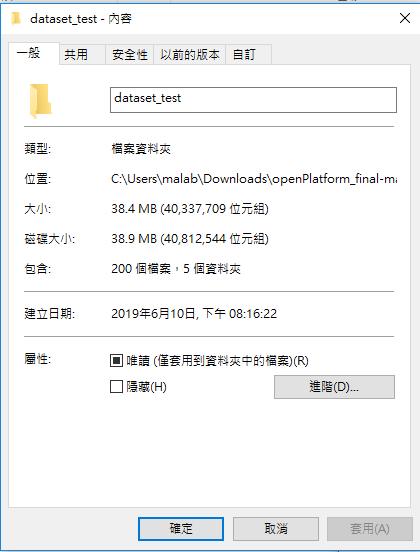
\includegraphics[height=4cm]{6.png}
\end{center}
\caption{所有類別的Test Data}
\end{figure}
\end{frame}
\section{Experimental Evaluation}
\subsection{Experimental environment (CPU, GPU, memory,…,etc.)}
\subsection{How many epochs you set for training?}
\subsection{Qualitative evaluation}
\subsection{Quantitative evaluation}



\end{CJK}
\end{document}


